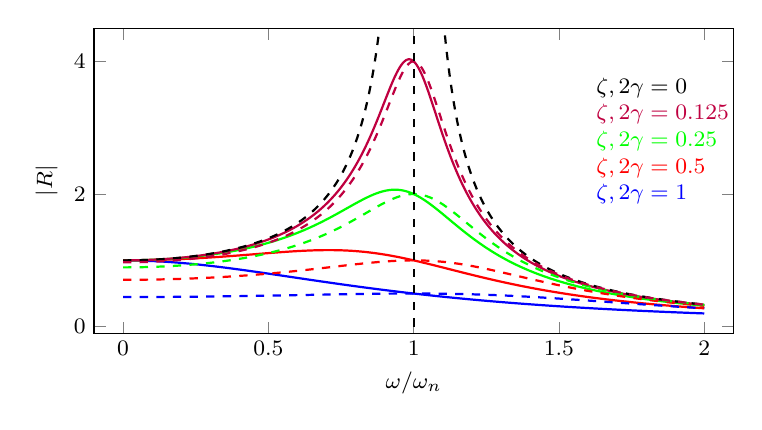
\begin{tikzpicture}[scale=1]
	\footnotesize
	\begin{axis}[
		width=0.8\textwidth,
		height=0.45\textwidth,
		xlabel={$\omega/\omega_n$},
		ylabel = {$|R|$},
		xmax=2.1,
		xmin=-0.1,
		ymax=4.5,
		ymin=-0.1,  
		samples=500]
		
		
		\def\k{1};
		\def\zetaA{1};
		\def\zetaB{0.5};
		\def\zetaC{0.25};
		\def\zetaD{0.125};		
		\def\zetaE{0.01};		
		
		\addplot[blue, thick, domain=0:2] (x, {1/sqrt(\k^2*(1-(x)^2)^2 + (\zetaA*2*\k*(x))^2)});
		\addplot[red, thick, domain=0:2] (x, {1/sqrt(\k^2*(1-(x)^2)^2 + (\zetaB*2*\k*(x))^2)});		
		\addplot[green, thick, domain=0:2] (x, {1/sqrt(\k^2*(1-(x)^2)^2 + (\zetaC*2*\k*(x))^2)});		
		\addplot[purple, thick, domain=0:2] (x, {1/sqrt(\k^2*(1-(x)^2)^2 + (\zetaD*2*\k*(x))^2)});		
		\addplot[black, dashed, thick, domain=0:2] (x, {1/sqrt(\k^2*(1-(x)^2)^2 + (\zetaE*2*\k*(x))^2)});		
		

		\addplot[blue, dashed, thick, domain=0:2] (x, {1/sqrt(\k^2*(1-(x)^2)^2 + (\zetaA*2*\k)^2)});
		\addplot[red, dashed, thick, domain=0:2] (x, {1/sqrt(\k^2*(1-(x)^2)^2 + (\zetaB*2*\k)^2)});		
		\addplot[green, dashed, thick, domain=0:2] (x, {1/sqrt(\k^2*(1-(x)^2)^2 + (\zetaC*2*\k)^2)});		
		\addplot[purple, dashed, thick, domain=0:2] (x, {1/sqrt(\k^2*(1-(x)^2)^2 + (\zetaD*2*\k)^2)});		


		
		\draw [thick, dashed] (axis cs: 1, 0) -- (axis cs: 1,5);
		
		\node at (axis cs: 1.6, 2) [blue,anchor=west] {$\zeta,2\gamma=1$};
		\node at (axis cs: 1.6, 2.4) [red,anchor=west] {$\zeta,2\gamma=0.5$};
		\node at (axis cs: 1.6, 2.8) [green,anchor=west] {$\zeta,2\gamma=0.25$};
		\node at (axis cs: 1.6, 3.2) [purple,anchor=west] {$\zeta,2\gamma=0.125$};
		\node at (axis cs: 1.6, 3.6) [black,anchor=west] {$\zeta,2\gamma=0$};
		
	\end{axis}
	
\end{tikzpicture}